% \documentclass{report}

% \usepackage{subcaption} % package for subfigures
% \usepackage{hyperref}  % package for linking figures etc
% \usepackage{enumitem}  % package for description with bullets
% \usepackage{graphicx}  % package for importing images
% \usepackage{mathtools} % package for math equation
% \usepackage{mathrsfs}  % package for math font
% \usepackage{indentfirst} % package for getting ident after section or paragraph
% \usepackage[export]{adjustbox}
% \usepackage{longtable} % package for multi pages tables
% \usepackage{multirow}  % package for tables, multirow
% \usepackage{esvect}
% % \usepackage{amsmath}

% \setlength{\parindent}{2em} % how much indent to use when we start a paragraph

% \graphicspath{ {./theory/figures/} }       % path for images

% \begin{document}

\chapter{Classification stage}
\section{Introduction}
In previous 2 chapters, we introduced the procedure we used to create
candidate action tubes, which probably contain some action or may not.
Most of the times, the proposed action tubes belong to the background, and for that reason, as mentioned
and in the previous chapter, it is important to choose a good linking algorithm that generates good sequences of bounding
boxes. However, it is quite important to choose the appropriate classifier who will be able
very accurately predict whether a candidate action tube belongs to a known category of actions or
it belongs to the background. This is because we may produce good proposals for candidate actions, but if our classier
is unable to distinguish them, our system will again fail to recognize the actions. \par

The right choice of a classifier is a big dilemma we are facing and we need to answer. However, this classifier will get as input
some activation maps in order to be classified. Therefore, apart from the good selection of classifier, equally, 
good choice of features is important, too. Finally, the training process of the classifier plays a major role in order to 
be able to generalize and to avoid overfitting situations. \par

For our implementation, we implement approaches including a Linear Classifier, 
a Recursive Neural Network (RNN) Classifier, a Support Vector Machine (SVM) Classifier and a Multilayer perceptron (MLP).
Additionally, we experiment using feature maps obtained from 3D RoiAlign using, also, avg or max pooling. Last but not least, we try to
find the right ratio between foreground and background action tubes including their total number needed during training stage
in order our classifier to perform efficiently.

\begin{figure}[h]
  % 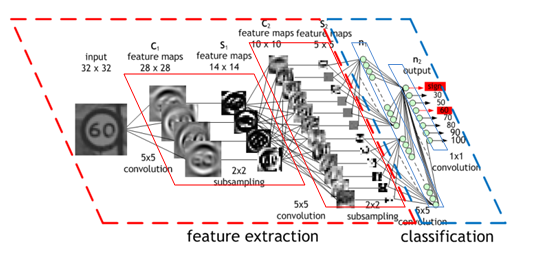
\includegraphics[scale=0.7]{convolutional_neural_network_structure} \]
  \centering
  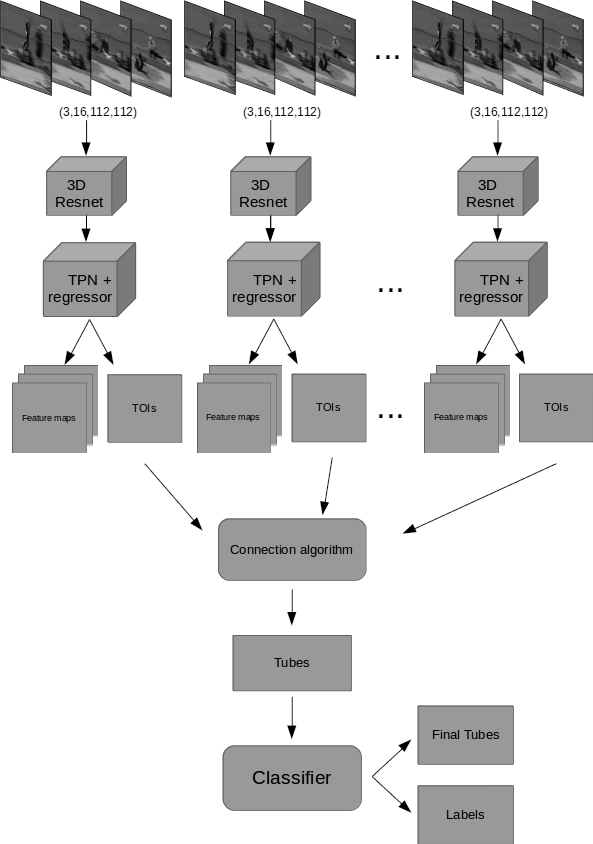
\includegraphics[scale=0.42]{model_withoutnms_v2}
  \caption{Structure of the whole network}
  \label{fig:whole_network}
\end{figure}

The whole procedure of classification is consisted from the following steps:
\begin{enumerate}
\item Separate video into small video clips and feed TPN network those video clips and get as output
  k-proposed ToIs and their corresponding features for each video clip.
\item Connect the proposed ToIs in order to get video tubes which may contain an action.
\item For each candidate video tube, which is a sequence of ToIs, feed its feature maps  into the classifier
  in order to perform classification.
\end{enumerate}

The general structure of the whole network is depicted in figure \ref{fig:whole_network}, in which we can see the aforementioned steps if we
follow the arrows.  \par
We treated each dataset seperately, because we didn't manage to achieve good recall performance for UCF-101 dataset, it is preferable to
experiment mainly at JHMDB dataset for spatiotemporal localization. Then, we performed temporal localization for UCF-101, because we achieve
good temporal recall performance during connection stage.

\section{Preparing data  and first classification results}

% \textbf{(Pending... Introduction about Linear and RNN classifiers)}
% \textbf{(Pending.. also an image of RNN classifier)}
For carrying out classification stage, we use, at first, a Linear classifier and a RNN classifier.
\paragraph{Linear Classifier} Linear classifier is a type of classifier which is able to discriminate objects and predict their
class based on the value of a \textit{linear combination} of object's feature values, which usually are presented in a feature
vector. If the input feature vector to the classifier is a real vector  $\vv{x}$, then the output score is :
\[ y = f(\vv{w} \cdot \vv{x}) = f \left( \sum_j w_jx_i \right) \]
\paragraph{RNN}
Recurrent neural networks, or RNNs for short, are a type of neural network that was designed to learn from sequence data,
such as sequences of observations over time, or a sequence of words in a sentence.
RNN takes many input vectors to process them and output other vectors.
It can be roughly pictured like in the Figure \ref{fig:rnn} below,
imagining each rectangle has a vectorial depth and other special hidden quirks in the image below.
For our case, we choose \textbf{many to one} approach, because we want only one prediction, at the end of
the action tube. \par
\begin{figure}[h]
  \centering
  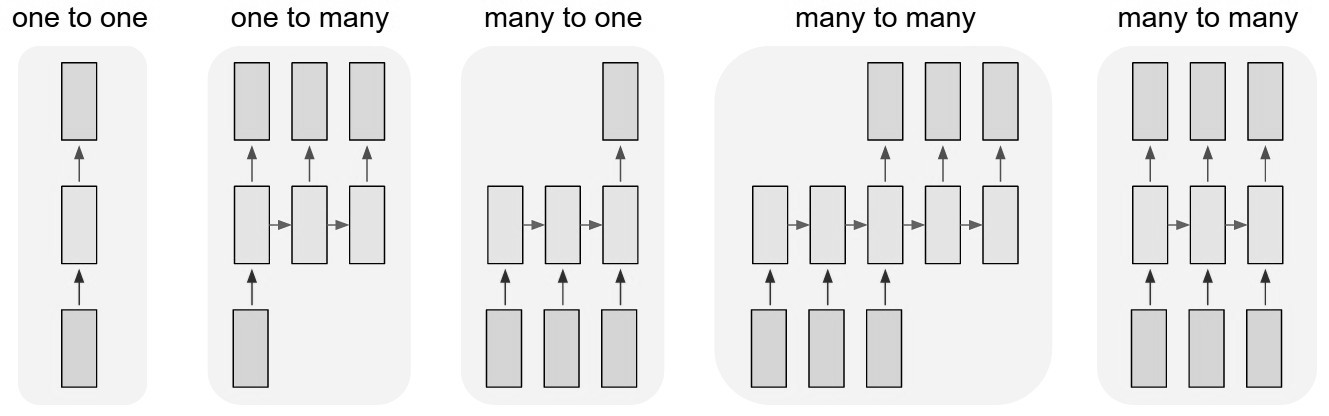
\includegraphics[width=1.\textwidth]{rnn.jpeg}
  \caption{Types of RNN}
  \label{fig:rnn}
\end{figure}

\paragraph{Training}
In order to train our classifier, we have to execute the steps, presented in the first section, for each video. However, each video
has different number of frames and reserves too much memory in the GPU. In order to deal with this situation and considering there are
4 GPUs available,
we give as input one video per GPU. So we can handle 4 videos simultaneously. This means that a regular
training session takes too much time for just 1 epoch. \par
The solution we came with, is to precompute the features for both foreground  and background video tubes, and 
then to feed those features to our classifier for training  it in order to discriminate classes. This solution includes the following steps:
\begin{enumerate}
\item  At first, we extract only groundtruth action tubes’ features. Also we extract feature maps from  background action tubes, which
  are double the number of groundtruth action tubes. We chose this
ratio between the number of  positive and negative tubes inspired by \cite{jjfaster2rcnn}, in which it has 25\% ratio between foreground
and background rois and chooses 128 roi in total. Respectively, we chose a little bigger ratio because we have only 1 groundtruth
video tube in each video. So, for each video we got 3 action  tubes in total, 1 for positive and 2 for background. We considered
background tubes those whose overlap scores with groundtruth tubes are $ \ge 0.1 $ and $ \le 0.3 $. Of course, 
in order to get those action tubes,we use a pre-trained TPN to generate ToIs for each video segment and then our proposed connection
algorithm for linking proposed ToIs. Finally, we get each action tube's corresponding feature map using 3D RoiAlign

\item After extracting those features, we trained both Linear and RNN classifiers. The Linear classifier needs a fixed input size, so
  we used a pooling function in the dimension of the number of videos. So, at first we had a feature map of \textit{3,512,16} dimensions and then
  we get as output a feature maps of \textit{512,16} dimensions. We experimented using  both max and avg pooling as shown at Table \ref{table:rnn_linear}.
  For the RNN classifier, we do not use any pooling function before feeding it.
\end{enumerate}
In order to train our classifiers, we use Cross-Entropy Loss as training loss function.
\paragraph{Validation} Validation stage includes using both pre-trained TPN and classifier. So, for each video,
we get classification scores for proposed action tubes. Most approaches usually consider a confidence score threshold for
considering an action tube as foreground. However, we don't use any confidence score. On the contrary, because we
know that JHMDB has trimmed videos with only 1 performed action, we just consider the best-scoring tube as our prediction.


\begin{table}[h]
  \centering
  \begin{tabular}{|| c | c || c  c  c ||}
    \hline
    \multirow{2}{*}{\textbf{Classifier}} & \multirow{2}{*}{\textbf{Pooling}} &  {} & \textbf{mAP} & {} \\
    {} & {} & 0.5 & 0.4 & 0.3 \\
    \hline
    \multirow{2}{*}{Linear} & mean & 14.18 & 19.81 & 20.02 \\
    \cline{2-5}
    {} & max & 13.67 & 16.46 & 17.02 \\
    \hline
    RNN  & -  & 11.3 & 14.14 & 14.84 \\
    \hline
  \end{tabular}
  \caption{First classification results using Linear and RNN classifiers}
  \label{table:rnn_linear}
\end{table}

  
% \textbf{(Pending results RNN... Table)}
% \textbf{(Pending results RNN... commentary)}
Table \ref{table:rnn_linear} shows first classification results, which are not very good. The only useful deduction that we can come with, using above results is that, avg pooling
method outclass max pooling. So, for all the rest classifications using Linear classifier, we use avg pooling before classification
stage.
% The results are disappointing.
% As we can see in the table, RNN classifier cannot classify very well because, probably, the duration of the videos are so small
% so we stopped using it in jHMDB dataset. In the Linear classifier, we noticed that every tube is considered as background tube.
% That means that Linear classifier gets overfitted with trained data and cannot handle unknown data. So, we thought that we
% need a classifier which can \"learn\" very easily, with little data. So we chose to try a support vector machine classifier.

\section{Support Vector Machine (SVM)}
SVMs are classifiers defined by a separating hyper-plane between trained data in a N-dimensional space. The main advantage of using a SVM
is that can get very good classification results when we have few data available. \par
The use of SVM is inspired from \cite{Girshick:2015:FR:2919332.2920125} and it is trained using hard negative mining. 
This means that we have 1 classifier per class which has only 2 labels, positive and negative. We mark as positive the feature maps of the
groundtruth action, and as negative groundtruth actions from other classes, and feature maps from background classes.
As we know, SVM is driven by small number of examples near decision boundary. Our goal is to find a set of negatives that are the closest to
the separating hyper-plane. So in each iteration, we update this set of negatives adding those which our SVM didn't perform very well. Each
SVM is trained independently. \par
SVM code is take from Microsoft's Azure \href{https://github.com/Azure/ObjectDetectionUsingCntk} {github page} in which there is an implementation
of Fast RCNN using a SVM classifier. We didn't modify its parameters which means that it has a linear kernel, uses  L2-norm as penalty and L1-norm
as loss during training. Training procedure starts with randomly picking 100 videos in order to calculate feature's scale.
After that, each svm is provided by positive samples' feature maps and network looks for hard negatives for each class' svm. We consider as hard-negatives the tubes
that got confidence score $ >  -1.0 $ during classification, and we add them to svm's samples. When we gather  hard-negatives whose number is bigger than 500 or 1000 (depending
on the approach) we retrain the class' SVM and remove samples with new score $ < -1.0$.  \par 
This whole process makes the choice of the negatives a crucial factor. In order to find the best policy,  we came with 5 different cases to consider
as negatives:
\begin{enumerate}
\item Negatives are other classes' positives and all the background tubes
\item Negatives are only all the background videos
\item Negatives are only other classes' positives
\item Negatives are other classes' positives and background tubes taken only from videos that contain a positive tube
\item Negatives are only background tubes taken from videos that contain a positive tube
\end{enumerate}

On top of that, we use 2 pooling functions in order to have a fixed input size. \par
In the next tables, we show our architecture's  mAP performance when we follow each one of the above policies. Also,
we experimented for 2 feature maps, \textit{(64,8,7,7)} and \textit{(256,8,7,7)} where 8 equals with the sample duration.
Both feature maps were extracted by using 3D RoiAlign procedure from feature maps with dimensions \textit{(64,8,28,28)} and
\textit{(256,8,7,7)} respectively (in the second case, we just add zeros in the feature map outsize from the bounding boxes for
each frame). Table \ref{table:svm_first_results} contains the first classification results. At first column we have the dimensions
of feature maps before pooling function, where k = 1,2,..5 . At second column we have feature maps' dimensions after pooling, and at
the next 2 column, the type of pooling function and the policy we followed. Finally in the last 3 columns we have the mAP performance
when we have threshold equal to 0.3, 0.4 and 0.5 respectively. During validation, we keep only the best scoring tube because we know that
we have only 1 action per video.

\begin{center}
\begin{longtable}{||c | c | c| c||c c c||}

  \hline
  \multicolumn{2}{||c|}{\textbf{Dimensions}} & \multirow{2}{*}{ \textbf{Pooling}} &\multirow{2}{*}{\textbf{Type}} & \multicolumn{3}{|c||}{\textbf{mAP precision}}\\

   before & after &  {} & {} &  0.5 &  0.4 & 0.3 \\
 \hline   \hline
 \multirow{5}{*}{(k,64,8,7,7)} & \multirow{5}{*}{(1,64,8,7,7)} & \multirow{5}{*}{mean}  & 1 &  3.16 & 4.2 & 4.4    \\
  \cline{4-7}
  {} & {} & {} & 2 & 2.29 & 2.68 & 2.86    \\
    \cline{4-7}
  {} & {} & {} & 3 & 1.63 & 3.16 &  4  \\
    \cline{4-7}
  {} & {} & {} & 4 & 2.42 & 4.83 & 5.46  \\  
    \cline{4-7}
  {} & {} & {} & 5 & 0.89 &1.12 & 1.21  \\
  \hline
 \multirow{5}{*}{(k,64,8,7,7)} & \multirow{5}{*}{(1,64,8,7,7)} & \multirow{5}{*}{max}  & 1 & 1.11 & 2.35 & 2.71 \\
    \cline{4-7}
  {} & {} & {} & 2 & 2.31 & 2.62 & 2.64 \\
    \cline{4-7}
  {} & {} & {} & 3 & 1.11 & 2.35 & 2.71 \\
    \cline{4-7}
  {} & {} & {} & 4 & 1.41 & 2.76 & 3.84  \\
    \cline{4-7}
  {} & {} & {} & 5 & 0.33 & 0.51 &0.58  \\

  \hline   \hline

 \multirow{5}{*}{(k,256,8,7,7)} & \multirow{5}{*}{(1,256,8,7,7)} & \multirow{5}{*}{mean}  & 1 &  11.41 & 11.73 & 11.73 \\

    \cline{4-7}
  {} & {} & {} & 2 & 10.35 & 10.92 &11.89 \\
    \cline{4-7}
  {} & {} & {} & 3 & 8.93 & 9.64 & 9.94 \\
    \cline{4-7}
  {} & {} & {} & 4 & 12.1 & 13.04 &13.04 \\
    \cline{4-7}
  {} & {} & {} & 5 & 5.92 & 6.92 & 7.79 \\
    \hline
 \multirow{5}{*}{(k,256,8,7,7)} & \multirow{5}{*}{(1,256,8,7,7)} & \multirow{5}{*}{max}  & 1  & \textbf{22.07} & \textbf{24.4} &  \textbf{25.77} \\
    \cline{4-7}
  {} & {} & {} & 2  & 14.07 & 16.56 & 17.74 \\
    \cline{4-7}
  {} & {} & {} & 3  & 14.22 & 18.94 &21.6 \\
    \cline{4-7}
  {} & {} & {} & 4  & 21.05 & 24.63 & 25.93 \\
    \cline{4-7}
  {} & {} & {} & 5  & 11.6 & 13.92 & 15.81 \\
  \hline   
  
  \caption{Our architecture's performance using 5 different policies and 2 different feature maps while pooling in
  tubes' dimension. With bold is the best scoring case}
  \label{table:svm_first_results}

\end{longtable} 
\end{center}

From the above results we notice that features map with dimension (256,8,7,7) outperform in all cases, both for mean and max pooling and
for all the policies. Also, we can see that max pooling outperforms mean pooling in all cases, too. Last but not least, we notice that policies
2, 3 and 5 give us the worst results which means that svm needs both data from other classes positives and from background tubes. 

\subsection{Modifying 3D Roi Align}
As we mentioned before, we extract from each tube its activation maps using 3D Roi Align procedure and we set equal to zero the pixels outside
of bounding boxes for each frame. We came with the idea that the environment surrounding the actor sometimes help us determine the class
of the action which is performed. This is base in the idea that 3D Convolutional Networks use the whole scene in order to classify the action
that is performed. We thought to extend a little each bounding box both in width and height. So, during Roi Align procedure, after resizing
the bounding box into the desired spatial scale  ( in our case 1/16 because original sample size = 112 and resized sample size = 7 )
we increase by 1 both width and height. According to that if we have a resized bounding box $( x_1,y_1,x_2,y_2) $ our new bounding box becomes
$ (max(0,x_1-0.5),max(0,y_1-0.5),min(7,x_2+0.5),min(7,y_2+0.5)) $ ( we use \textit{ min} and \textit{max} functions in order to avoid exceeding feature maps' limits).
We just experiment in policies 1 and 4 for both (256,8,7,7) and (64,8,7,7) feature maps as show in  Table \ref{table:svm_mod_roialign}


\begin{center}
\begin{longtable}{||c | c | c| c||c c c||}

  \hline
  \multicolumn{2}{||c|}{\textbf{Dimensions}} & \multirow{2}{*}{ \textbf{Pooling}} &\multirow{2}{*}{\textbf{Type}} & \multicolumn{3}{|c||}{\textbf{mAP precision}}\\

   before & after &  {} & {} &  0.3 &  0.4 & 0.5 \\
 \hline   \hline
 \multirow{2}{*}{(k,64,8,7,7)} & \multirow{2}{*}{(1,64,8,7,7)} & \multirow{2}{*}{mean}  & 1 & 9.75 & 11.92 & 13.34 \\
  \cline{4-7}
  {} & {} & {} & 4 &  5.74 &6.62 & 7.59 \\
  \hline
 \multirow{2}{*}{(k,64,8,7,7)} & \multirow{2}{*}{(1,64,8,7,7)} & \multirow{2}{*}{max}  & 1 &  6.46 & 10.26 & 10.83 \\
    \cline{4-7}
  {} & {} & {} & 4 & 4.19 & 6.27 & 7.52 \\
    \cline{4-7}
  \hline
  \caption{Our architecture's performance using 2 different policies and 2 different pooling methods using modified Roi Align.}
  \label{table:svm_mod_roialign}

\end{longtable} 
\end{center}

According to Table \ref{table:svm_mod_roialign}, modified Roi Align doesn't improve mAP performance. On the contrary, it reduces it.
However, the gap between those 2 approaches is small, so we don't abandon this idea, because, for different approaches,
modified Roi Align may outclass regular Roi Align.

\subsection{Temporal pooling}
After getting first results, we implement a temporal pooling function inspired from \cite{DBLP:journals/corr/HouCS17}. We need a
fixed input size for the SVM. However, our tubes' temporal stride varies from 2 to 5, because a video lasting 15 frames
is consisted of 2 ToIs and a video of 40 frames is consisted of 5. So we use as fixed temporal pooling equal
with 2. As pooling function we use 3D max pooling, one for each filter of the feature map.  So for example, for an action tube
with 4 consecutive ToIs, we  have $(4,256,8,7,7)$ as feature size. We separate the feature map into 2 groups using \textit{linspace}
function and we reshape the feature map into $(256,k,8,7,7)$ where k is the size of each group. After using 3D max pooling, we get
a feature map with dimensions $(256,8,7,7)$, so we concat them and finally get feature maps with size of $(2,256,8,7,7)$.
In this case we didn't experiment with feature maps with size $(64,8,7,7)$ because they wouldn't performed better than  feature maps with size $(256,8,7,7)$ as noticed from the previous section. \par
We experiment using a SVM classifier for training policies 1 and 4 and using both regular and modifier Roi Align. The
performance results are presented at Table \ref{table:svm_temp_pooling}.
% \newpage
\begin{center}
\begin{longtable}{||c | c| c| c||c c c||}

  \hline
 \multicolumn{2}{||c|}{\textbf{Dimensions}} & \multirow{2}{*}{\textbf{Pooling}} &\multirow{2}{*}{ \textbf{Type}} &\multicolumn{3}{|c||}{\textbf{mAP precision}}\\

  before & after & {} & {} & 0.5 &  0.4 & 0.3\\
  \hline   \hline

  \multirow{4}{*}{k,256,8,7,7} & \multirow{4}{*}{2,256,8,7,7} & \multirow{2}{*}{RoiAlign}  & 1 & 24.97 & 26.91 & 29.11 \\
  \cline{4-7}
  {} & {} & {} & 4 &  23.27 & 25.96 & 28.25 \\
  \cline{3-7}
  {} & {} & \multirow{2}{*}{mod RoiAlign} & 1 & 7.01 & 9.69 & 10.52 \\
  \cline{4-7}
  {} & {} & {} & 4 & 5.5 & 7.25 & 8.99 \\
  \hline

  \caption{mAP results using temporal pooling for both RoiAlign approaches}
  \label{table:svm_temp_pooling}
\end{longtable} 
\end{center}

Comparing Tables \ref{table:svm_mod_roialign} and \ref{table:svm_temp_pooling}, we clearly notice that we get better results when
using temporal pooling. Also, the difference between regular Roi Align and modified Roi Align become much bigger than previously,
so this makes us abandon the idea of modified Roi Align. So, the rest section, we only experiment using regular Roi Align.

\section{Increasing sample duration to 16 frames}

Next, we though that a good idea would be to increase the sample duration from 8 frames to 16 frames. We experiment both using and not
using temporal pooling, again for policies 1 and 4. Results are included at table \ref{table:svm_temp_pooling_16}. 

\begin{center}
\begin{longtable}{||c | c| c| c||c c c||}

  \hline
 \multicolumn{2}{||c|}{\textbf{Dimensions}} & \multirow{2}{4.5em}{\textbf{Temporal Pooling}} &\multirow{2}{*}{ \textbf{Type}} &\multicolumn{3}{|c||}{\textbf{mAP precision}}\\

  before & after & {} & {} &  0.5 &  0.4 & 0.3 \\
  \hline   \hline

  \multirow{2}{*}{k,256,16,7,7} & \multirow{2}{*}{1,256,16,7,7} & \multirow{2}{*}{No}  & 1 & 23.4 & 27.57 &28.65  \\
  \cline{4-7}
  {} & {} & {} & 4 & 22.7 & 26.95 & 28.05 \\
  \hline

  \multirow{2}{*}{k,256,16,7,7} & \multirow{2}{*}{2,256,16,7,7} & \multirow{2}{*}{Yes}  & 1 & 21.12 & 24.07 & 24.36  \\
  \cline{4-7}
  {} & {} & {} & 4 & 18.36 & 23.09 & 23.75 \\
  \hline
  \caption{mAP results for  policies 1,4  for sample duration = 16 }
  \label{table:svm_temp_pooling_16}
\end{longtable} 
\end{center}

As shown at Table \ref{table:svm_temp_pooling_16}, we get better performance when we don't use temporal pooling, fact that is unexpected.
However, the difference between those performances is about 2\%. Probably, this is caused by the fact that, in the temporal pooling approach,
SVM classifier has to train too many parameters when it uses temporal pooling, on the contrary with the approach not using temporal pooling,
in which SVM has to train half the number of parameters. Furthermore, comparing above results with results shown at Table  \ref{table:svm_mod_roialign}, we can see that we get about the same results for both approaches. So, we choose to keep using approach with sample duration equal
with 8. That's because, we don't have to use too much memory during training and validation.

\section{Adding more groundtruth tubes}
% \textbf{Pending more comments...} \\
% From above results, we notice that SVM improve a lot the performance of our model. In order to further improve our results, we will
% add more groundtruth action tubes. We consider as groundtruth action tubes all the tubes whose overlap score  with a groundtruth tube is
% greater that 0.7 . Also, we increase the total number of tube to from 1 to 2, 8. Table \ref{table:svm_increased}

The previous results came from when we train classifiers using only 1 groundtruth action tube and 2 background. We thought that we should
experiment with the number of foreground action tubes and the ratio between foreground and background tubes because in previous approaches
these numbers were a little arbitrary. So, we choose to train our previous classifiers using 2, 4 and 8 foreground tubes and a ratio of 2:3,
1:2, 1:3, and 1:4 between the number of foreground tubes and the total number of both foreground and background tubes. \par

Firstly, we train the RNN classifier using feature maps with dimensions \textit{(256,8,7,7)} and mAP performance is presented at Table 
\ref{table:rnn_increased} for overlap threshold equal to 0.5, 0.4 and 0.3 . 
% \begin{table}[h]
%   \centering
%   \begin{tabular}{|| c | c | c || c c c||}

\begin{center}
  \begin{longtable}{|| c | c | c || c c c||}
    \hline
    \multirow{2}{*}{\textbf{F. map}} & \multirow{2}{*}{\textbf{FG tubes}}  & \multirow{2}{*}{\textbf{Total tubes}} & {} & \textbf{mAP} & {} \\
    {}  & {} & {} & 0.5 & 0.4 & 0.3 \\
    \hline
    \multirow{7}{*}{(k,256,8,7,7)} & 1 & 3 & 11.3 & 14.14 & 14.84 \\
    \cline{2-6}
    {} & \multirow{4}{*}{2} & 3 & 1.96 & 5.07 & 7.27 \\
    \cline{3-6}
    {} & {} & 4  & 3 & 5.03 & 5.77 \\
    \cline{3-6}
    {} & {} & 6 & 1.34 & 3.89 & 4.49 \\
    \cline{3-6}
    {} & {} & 8 & 0.77 & 1.51 & 2.72 \\
    \cline{2-6}
    {} & \multirow{4}{*}{4} &  6 & 13.23 & 21.74 & 25.4 \\
    \cline{3-6}
    {} & {} & 8 & 20.73 & 28.25 & 29.50 \\
    \cline{3-6}
    {} & {} & 12  & 16.55 & 24.35 & 25.22 \\
    \cline{3-6}
    {} & {} & 16  & 20.11 & 25.50 & 27.62 \\
    \cline{2-6}
    {} & \multirow{4}{*}{8} & 12 & 13.82 & 19.93 & 22.80 \\
    \cline{3-6}
    {} &  {} & 16 & 15.47 & 23.08 & 24.19 \\
    \cline{3-6}
    {} &  {} & 24 & 15.88 & 23.44 & 24.48  \\
    \cline{3-6}
    {} &  {} & 32 &  12.66 & 23.50 & 25.61 \\
    \hline

  \caption{RNN results }
  \label{table:rnn_increased}
\end{longtable}
\end{center}

According to Table \ref{table:rnn_increased}, firstly we can see that increasing the number of foreground tubes from 1 to 2 leads to reduce
rapidly mAP performance. But, when we set foreground tubes equal to 4 we get better results. On top of that, we get best performance when
the ratio is equal to 1:2 and 1:4. Finally, when we set the number of foreground tubes equal to 8, performance gets slightly better
comparing with the initial conditions (1 foreground action tube and 3 in total) but, this situation doesn't get us the best results. \par 
Next, it's time to experiment using the Linear classifier. We use again the same cases like we did for RNN classification. As mentioned
before, we need a pooling method before classification step. According to Table \ref{table:rnn_linear}, avg pooling method results in
better mAP performance than max pooling, so we use avg pooling for all following cases. Results are included at Table \ref{table:linear_increased}.

\begin{center}
  \begin{longtable}{|| c | c | c || c c c||}
    \hline
    \multirow{2}{*}{\textbf{F. map}} & \multirow{2}{*}{\textbf{FG tubes}} & \multirow{2}{*}{\textbf{Total tubes}} & {} & \textbf{mAP} & {} \\
    {}  & {} & {} & 0.5 & 0.4 & 0.3 \\
    \hline
    \multirow{7}{*}{(k,256,8,7,7)}  & 1 & 3& 14.18 &19.81 & 20.02 \\
    \cline{2-6}
    {} & \multirow{4}{*}{2} & 3 & 12.68 & 13.38 & 15.14 \\
    \cline{3-6}
    {} & {} & 4 & 11.5 & 14.95 & 16.22 \\
    \cline{3-6}
    {} & {} & 6 & 10.74 & 13.36 & 15.18 \\
    \cline{3-6}
    {} & {} & 8 & 8.00 & 9.83 & 11.17 \\
    \cline{2-6}
    {} & \multirow{4}{*}{4} & 6 & 15 & 17.55 & 19.39 \\
    \cline{3-6}
    {} & {} & 8 & 17.04	& 20.12 &22.07 \\
    \cline{3-6}
    {} & {} & 12 & 17.57 & 19.9 & 21.88 \\
    \cline{3-6}
    {} & {} & 16 & 14.24 & 17.24 & 17.95 \\

    \cline{2-6}
    {} & \multirow{4}{*}{8} & 12 & 17.91 & 22.51 & 24.62 \\
    \cline{3-6}
    {} & {} & 16 & 16.76 & 20.34 & 22.72 \\
    \cline{3-6}
    {} & {} & 24 & 17.61 & 19.12 & 24.48 \\
    \cline{3-6}
    {} & {} & 32 & 14.45 & 18.07 & 19.14  \\
    \hline

    \caption{Linear results }
    \label{table:linear_increased}
  \end{longtable}
\end{center}

First of all, after considering results presented at both Tables \ref{table:rnn_increased} and \ref{table:linear_increased}, it becomes clear that when we
set the number of foreground tubes equal to 2, for both case, we get worse results that the initial. This probably is due to the fact that we increase
also the number of background tubes for cases when ratio is 1:2, 1:3 and 1:4 resulting in considering more proposed tubes as background tubes. On the other
hand when we set ratio equal to 2:3, instead of considering most proposed action tubes as background, classifiers classify them as a specific action class,
which means there is an overfitting situation. So, although we think that we shouldn't investigate any more for cases with 2 foreground action tubes,
we will train our SVM classifier using 2 foreground tubes and all the aforementioned ratio because we want to be sure about our assumption. On the other hand
we notice that using 4 or 8 foreground tubes both  get us better results than the initial results. The best results come when  ratio between foreground and
total tubes is 1:3 for both cases. Furthermore, we get good results for ratios 2:3 and 1:2, and we get the worst while using ratio 1:4. This is caused probably
from the big number of background tubes comparing with the one of foreground tubes. \par 
As mentioned before, we train SVM classifier using aforementioned cases only for policy 1 because it gives us the best results for all previous cases.
Classification performance using mAP metric is shown at Table \ref{table:svm_increased}. 

\begin{center}
  \setlength{\tabcolsep}{2pt}
  \begin{longtable}{|| c | c | c || c c c||}


    \hline
    \multirow{2}{*}{\textbf{F. map}} & \multirow{2}{*}{\textbf{FG tubes}} & \multirow{2}{*}{\textbf{Total tubes}} & {} & \textbf{mAP} & {} \\
    {}  & {} & {} & 0.5 & 0.4 & 0.3 \\
    \hline
    \multirow{8}{*}{(2,256,8,7,7)} & 1 & 3 & 24.97 & 26.91 & 29.11\\
    \cline{2-6}
    {} & \multirow{4}{*}{2} & 3 & 13.87 & 18.74 & 21.29 \\
    \cline{3-6}
    {} & {} & 4 & 14.21 & 19.67 & 21.75 \\
    \cline{3-6}
    {} & {} & 6 & 12.88 & 18.62 & 21.59 \\
    \cline{3-6}
    {} & {} & 8 & 12.66 & 18.7 & 21.97 \\
    \cline{2-6}
    {} & \multirow{4}{*}{4} & 6 & 25.04 & 26.91 & 27.82  \\
    \cline{3-6}
    {} & {} &  8 & 24.34 & 25.67 & 26.34 \\
    \cline{3-6}
    {} & {} & 12 &  23.47 & 25.31 & 25.9 \\
    \cline{3-6}
    {} & {} & 16 & 21.94 & 23.55 & 24.23 \\
    \cline{2-6}
    {} & \multirow{4}{*}{8} & 12 & 24.83 & 27.13 & 27.46 \\
    \cline{3-6}
    {} & {} & 16 & 23.97 & 26.38 & 26.94 \\
    \cline{3-6}
    {} & {} & 24 & 24.17 & 26.24 & 26.76 \\
    \cline{3-6}
    {} & {} & 32 & 24.17 & 26.24 & 26.76 \\

    \hline

    \caption{SVM results }
    \label{table:svm_increased}
  \end{longtable}
\end{center}

Results shows us some interesting facts. Firstly, it confirms our assumption that our network is unable to train well with only 2 foreground tubes, so from now on,
we will investigate training situations using 4 or 8 foreground action tube during training. Also, a strange fact occurs, which is that we get almost the
same results with the results obtained for using policy 1, only one foreground tube, 3 in total and temporal pooling. This is probably because
during calculation of feature scale, during training stage, we don't get such good sample set of video like we did during aforementioned situation. But we think that it is better to
keep testing using 4 or 8 foreground action tubes. Last but not least, it is clear that we get the best result when we have ratio 2:3 between
number of foreground and total action tubes. Also, it is more preferable to have 4 foreground action tubes instead of 8. This means that given too
many action tubes confuse SVM classifier, so it fails to perform well.


\subsection{Increasing again sample duration (only for RNN and Linear)}

Table \ref{table:svm_temp_pooling_16} showed that SVM classifier gets about the same performance for both sample durations 8 and 16 frames.
Triggered by this fact, we trained RNN and Linear classifiers for sample duration equal to 16 frames. Table \ref{table:rnn_16} shows RNN's mAP
performance and Table \ref{table:linear_16} Linear's mAP performance. We started experimenting with RNN classifier because it performed better than
Linear classifier previously. As mentioned before, we experiment using 4 or 8 foreground tubes and ratios 2:3, 1:2, 1:3 and 1:4 between the number of
foreground and total action tubes provided.

\begin{center}
  \begin{longtable}{|| c | c || c c c ||}
    \hline
    \multirow{2}{*}{\textbf{FG tubes}} & \multirow{2}{*}{\textbf{Total tubes}} & {} & \textbf{mAP} & {} \\
    {} & {} & 0.5 & 0.4 & 0.3 \\
    \hline
    \multirow{4}{*}{4} & 6 & 7.94 & 13.51 & 14.95 \\
    \cline{2-5}
    {} & 8 & 10.88 & 14.02 & 14.74  \\
    \cline{2-5}
    {} & 12 & 14.05 & 19.23 & 20.99 \\
    \cline{2-5}
    {} & 16 & 11.69 & 15.77 & 16.87  \\
    \hline
    \multirow{4}{*}{8} & 12 & 10.47 & 15.06 & 19.93 \\
    \cline{2-5}
    {} & 16 &  12.29 & 19.51 & 23.11  \\
    \cline{2-5}
    {} & 24 & 12.85 & 18.35 & 20.00 \\
    \cline{2-5}
    {} & 32 & 9.38 & 14.33 & 16 \\
    \hline

  \caption{RNN results for sample duration equal to 16}
  \label{table:rnn_16}
\end{longtable}
\end{center}

Comparing results from Table \ref{table:rnn_16} and previous table \ref{table:rnn_increased} one by one, it is clear that RNN outperforms when sample
duration equals with 8 frames. This results was expected, because, the increase of sample duration reduce the number of video segments needed for each video.
So, this means that RNN has to classify sequences with 3 video segments at the most, which is more difficult that classifying bigger sequence like previously. \par
Next, we experiment using Linear classifier for the same cases like RNN's. 

\begin{center}
  \begin{longtable}{|| c | c || c c c ||}
    \hline
    \multirow{2}{*}{\textbf{FG tubes}} & \multirow{2}{*}{\textbf{Total tubes}} & {} & \textbf{mAP} & {} \\
    {} & {} & 0.5 & 0.4 & 0.3 \\
    \hline
    \multirow{4}{*}{4} & 6 & 13.79 & 19.75 & 23.63 \\
    \cline{2-5}
    {} & 8 & 15.11 & 19.78 & 21.14 \\
    \cline{2-5}
    {} & 12 & 11.39 & 15.74 & 18.15 \\
    \cline{2-5}
    {} & 16 & 13.62 & 16.11 & 18.15 \\
    \hline
    \multirow{4}{*}{8} & 12 & 10.63 & 19.37 & 21.65 \\
    \cline{2-5}
    {} & 16 & 12.98 & 17.52 & 19.10 \\
    \cline{2-5}
    {} & 24 & 12.92 & 17.64 & 19.95 \\
    \cline{2-5}
    {} & 32 & 11.51 & 13.98 & 14.82 \\
    \hline

  \caption{Linear results for sample duration equal to 16}
  \label{table:linear_16}
\end{longtable}
\end{center}


In this case, results from table \ref{table:linear_16} are worse than  those presented at Table \ref{table:linear_increased}, with the difference being about 2\%.
So, after considering both cases, it becomes clear that it is preferable to experiment using sample duration equal to 8 and not to increase it to 16 frames.


\section{MultiLayer Perceptron (MLP)}

\begin{figure}[h]
  % 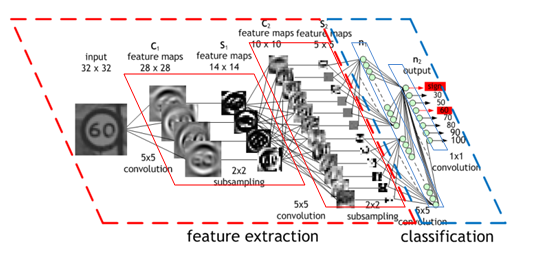
\includegraphics[scale=0.7]{convolutional_neural_network_structure} \]
  \centering
  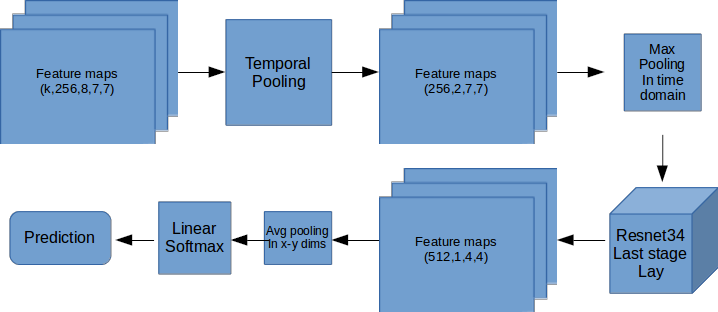
\includegraphics[scale=0.42]{mlp}
  \caption{Structure of the MLP classifier}
  \label{fig:mlp_structure}
\end{figure}

In previous sections we used classic classifiers like Linear, RNN and SVM. Last but not least,
another widely category of classifiers  is Multilayer Perceptron (MLP) classifiers. MLP is a class of
feedforward Neural Network, so its function is described in chapter 2.
So, we design a MLP which is shown in Figure \ref{fig:mlp_structure} for sample duration equal to 8, and is described below:
\begin{itemize}
\item At first,  after 3D Roi align and for sample duration = 8, we get an activation map of $(k,256,8,7,7)$ where $k$ is the
  number of linked ToIs. Inspired by previous sections, we perform temporal pooling followed by a max pooling operation in
  sample duration's dimension. So, we now have an activation maps with dimensions equal to $(2,256,7,7),$ which we reshape
  it into $(256,2,7,7)$  which we feed to 
 layers  extracted from the last stage of ResNet34. This stages includes 3 Residual Layers
  with stride equal to 2 in all 3 dimensions and output number of filters equal to 512.

\item After Residual Layers, we perform avg pooling for x-y dimensions. So we get as output activation maps with dimension size
  equal to (512,).  Finally, we feed these feature maps to a linear layer in order to get class confidence score, after applying
  soft-max function.

\end{itemize}

\subsection{Regular training}
According to figure \ref{fig:whole_network}, the trainable parts of our network is TPN and the classifier.
% At first, we tried to
% simultaneously train them, but, we got OutOfMemory errors during training, even thought we tried several modifications in our code.
% So, we came with the idea of, first training seperately TPN, according to chapter 4 and then train the whole network by freezeing
% TPN's layers. 
As mentioned before, training code requires running only one video per GPU, because, videos have different duration. For previous approaches
we came with the idea of pre-calculating video features and then training only the classifier. However, for this step, we normally trained our
in order to get classification results. Of course, we used a pre-trained TPN, whose layers were frozen in order not to be trained.
We tried to explore different ratios between the number of foreground tubes and the total number of tubes per video. First 3 simulations included
fixed number of total tubes and variable ratio between the number of foreground and background tubes. We started using only foreground tubes, which
means 32 out 32 tubes are foreground, then half of the proposed tubes aka 16 out of 32 and finally less than half, namely 14 out of 32. After that,
we experiment using a fixed number of foreground tubes and variable number of total tubes, which are 16, 24 and 32. The performance results are presented
at Table \ref{table:mlp_reg}.

\begin{center}
  \begin{longtable}{|| c | c || c c c ||}
    \hline
    \multirow{2}{*}{\textbf{FG tubes}} & \multirow{2}{*}{\textbf{Total tubes}} & {} &  \textbf{mAP} & {} \\
    {} & {} & 0.5 & 0.4 & 0.3 \\
    \hline
    32 & \multirow{3}{*}{32} &1.28 & 1.73 & 1.87  \\
    \cline{1-1} \cline{3-5}
    16 & {} & 3.98 & 4.38 & 4.38  \\
    \cline{1-1} \cline{3-5}
    14 & {} & 0.40 & 0.40 & 0.40 \\
    \hline
    \multirow{3}{*}{8} & 16 & 9.41 & 12.59 & 14.61 \\
    \cline{2-5}
    {} & 24 & 12.32 & 15.53 & 18.57 \\
    \cline{2-5}
    {} & 32 & 7.16 & 10.92 & 13.00 \\
    \hline
    \caption{MLP's mAP performance for regular training procedure}
    \label{table:mlp_reg}
  \end{longtable}
\end{center}

The results show that when first 3 approaches give us very bad results. Comparing them with the rest 3, we came with the conclusion that we
need at the most 8 foreground tubes, even thought the ratio between the number of foreground and background is in favor the second one.
Probably, too many foreground action tubes make our architecture overfitted so unable to generalize.

\subsection{Extract features}

As previously performed, we trained MLP classifier using pre-computed feature maps. These feature maps include both foreground and background
action tubes. Based on the conclusions made in previous sections, we will train our classifier only for number of foreground tubes equal to 4
and 8. Furthermore, we will train it for 3 different ratios between the number of foreground and background action tubes, which are 1:1, 1:2
and 1:3. Table \ref{table:mlp_extract_jhdmb} shows these cases and their respective mAP performance during validation step.

\begin{center}
  \begin{longtable}{|| c | c || c c c ||}
    \hline
    \multirow{2}{*}{\textbf{FG tubes}} & \multirow{2}{*}{\textbf{Total tubes}} & {} & \textbf{mAP} & {} \\
    {} & {} & 0.5 & 0.4 & 0.3 \\
    \hline
    \multirow{3}{*}{4} & 6 & 4,37 & 8,54 & 10,12 \\
    \cline{2-5}
    {} & 8 & 5.89 & 9.54 & 13.61 \\
    \cline{2-5}
    {} & 12 & 9.51 & 12.8 & 14.6  \\
    \cline{2-5}
    {} & 16 & 6.80 & 13.17 & 14.67 \\
    \hline
    \multirow{4}{*}{8} & 12 & 8,62 & 12,32 & 14,74 \\
    \cline{2-5}
    {} & 16 & 8.49 & 13.94 & 15.09 \\
    \cline{2-5}
    {} & 24 & 6.72 & 12.17 & 15.30 \\
    \cline{2-5}
    {} & 32 & 13.27 & 17.64 & 18.97 \\
    \hline

  \caption{mAP results for MLP trained using extracted features}
  \label{table:mlp_extract_jhdmb}
\end{longtable}
\end{center}

Comparing results from Tables  \ref{table:mlp_extract_jhdmb}  and \ref{table:mlp_reg}, it is clear we need 8 foreground tubes in order MLP
classifier to perform well. However, it isn't very
clear which of these two proposed training approaches is better, but if we have to decide one method, we would choose using pre-extracted features training.  This approach manages
to achieve the best results, and especially when we have 8 foreground action tubes and 32 in total. Also, comparing methods using 4 or 8 positive action tubes, it is clear that we
would prefer using 8 generally. However, it's not clear which ratio is better because, we get best results when we have 8 foreground action tubes  and  ratio 1:4 while we get best results
when ratio is 1:3 having 4 positive action tubes.

\section{Adding nms algorithm}

After getting previous classification results, we came with the idea that a lot of proposed action tubes overlap spatiotemporally like presented in chapter 4,
for the first linking algorithm. On top of that, even though, at last, we will keep only the best scoring action tube, maybe, our Network sometimes
doesn't score the best overlapping action tube but a neighbor, which should have been removed. So, similar with chapter 4, we added NMS algorithm
before classification stage in order to remove unnecessary overlapping action tubes.
The structure of this approach is presented at Figure \ref{fig:network_nms}. So, we run again validation stage for our classifiers
and results are presented at Tables \ref{table:svm_nms}, \ref{table:rnn_nms}, \ref{table:linear_nms} and \ref{table:mlp_nms} for SVM, RNN, Linear
and MLP classifiers respectively. \par

We start experimenting using SVM classifier, whose mAP performance is presented at Table \ref{table:svm_nms} when we use NMS algorithm.

\begin{figure}[h]
  % 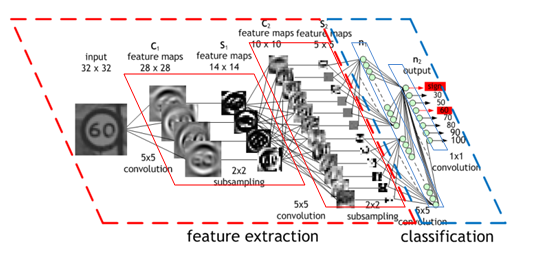
\includegraphics[scale=0.7]{convolutional_neural_network_structure} \]
  \centering
  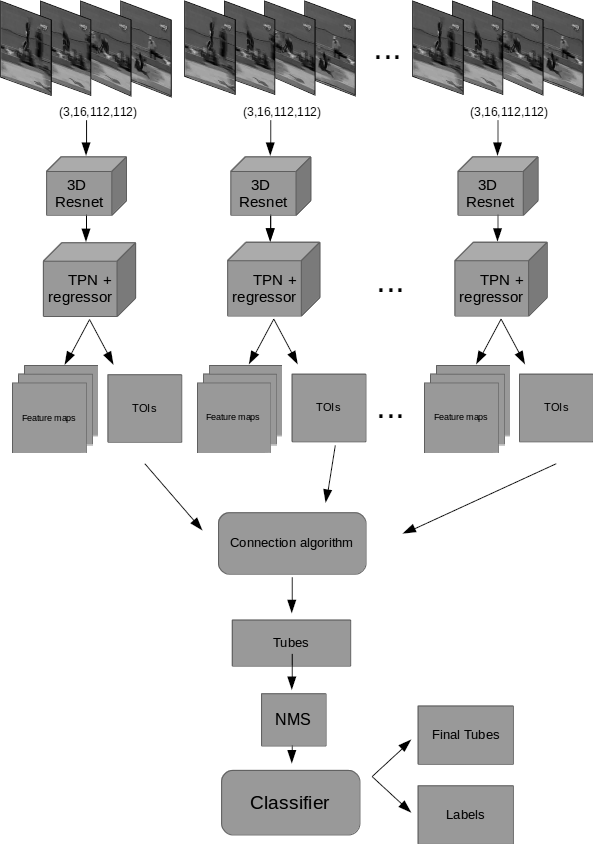
\includegraphics[scale=0.4]{model_withnms}
  \caption{Structure of the network with NMS}
  \label{fig:network_nms}
\end{figure}

\begin{center}
  \begin{longtable}{|| c | c || c c c ||}
    \hline
    \multirow{2}{*}{\textbf{FG tubes}} & \multirow{2}{*}{\textbf{Total tubes}} & {} & \textbf{mAP} & {} \\
    {} & {} & 0.5 & 0.4 & 0.3 \\
    \hline
    \multirow{4}{*}{4} & 6 & 21.42 & 24.3 & 25.11 \\
    \cline{2-5}
    {} & 8 & 21.3 & 24.06 & 24.85 \\
    \cline{2-5}
    {} & 12 & 21.73 & 24.19 & 25.04 \\
    \cline{2-5}
    {} & 16 & 21.11 & 23.98 & 24.84 \\
    \hline
    \multirow{4}{*}{8} & 12 & 20.47 & 22.55 & 23.41 \\
    \cline{2-5}
    {} & 16 & 21.21 & 23.89 & 24.97 \\
    \cline{2-5}
    {} & 24 & 21.71 & 23.8 & 24.82 \\
    \cline{2-5}
    {} & 32 & 21.43 & 23.5 & 24.52 \\
    \hline

  \caption{mAP results for SVM classifier after adding NMS algorithm}
  \label{table:svm_nms}
\end{longtable}
\end{center}

According to Table \ref{table:svm_nms} and taking Table's \ref{table:svm_increased} results into consideration, it is clear that mAP performance decreases while using NMS algorithm.
We run only for case with foreground tubes equal to 4 or 8 and we didn't experiment using initial ratio, because we think that we are going to get the same attitude.
This is probably because NMS algorithm removes some overlapping action tubes, so SVM classifier doesn't get the right action tubes for classifying them. \par

Next, we experiment using RNN classifier for sample duration equal to 8 frames per video segment. Results are included at Table \ref{table:rnn_nms}

\begin{center}
  \begin{longtable}{|| c | c || c c c ||}
    \hline
    \multirow{2}{*}{\textbf{FG tubes}} & \multirow{2}{*}{\textbf{Total tubes}} & {} & \textbf{mAP} & {} \\
    {} & {} & 0.5 & 0.4 & 0.3 \\
    \hline
    \multirow{4}{*}{4} & 6 & 13.27 & 26.12 & 30.69  \\
    \cline{2-5}
    {} & 8 & 16.06 & 25.81 & 27.63 \\
    \cline{2-5}
    {} & 12 & 13.93 & 22.48 & 23.99 \\
    \cline{2-5}
    {} & 16 & 17.24 & 26.44 & 28.36 \\
    \hline
    \multirow{4}{*}{8} & 12 & 2 & 5.11 & 7.75 \\
    \cline{2-5}
    {} & 16 & 11.11 & 20.98 & 23.97 \\
    \cline{2-5}
    {} & 24 & 13.84 & 22.77 & 24.31 \\
    \cline{2-5}
    {} & 32 & 12.74 & 21.49 & 25.39 \\
    \hline

  \caption{mAP results for RNN classifier after adding NMS algorithm}
  \label{table:rnn_nms}
\end{longtable}
\end{center}

Alongside with SVM's mAP performances, RNN doesn't achieve any improvement in its mAP performance when adding NMS algorithm. On the contrary, it reduce about 5\% in some cases, so it is more
preferable to use ActionNet's architecture without NMS algorithm included while using RNN as classifier. \par
Following RNN, we investigate the same situations with Linear classify instead of RNN. Its performance is presented at Table \ref{table:linear_nms}.

\begin{center}
  \begin{longtable}{|| c | c || c c c ||}
    \hline
    \multirow{2}{*}{\textbf{FG tubes}} & \multirow{2}{*}{\textbf{Total tubes}} & {} & \textbf{mAP} & {} \\
    {} & {} & 0.5 & 0.4 & 0.3 \\
    \hline
    \multirow{4}{*}{4} & 6 & 12.59 & 14.91 & 17.79  \\
    \cline{2-5}
    {} & 8 & 15.89 & 21.92 & 23.28 \\
    \cline{2-5}
    {} & 12 & 13.23 & 19.72 & 23.17 \\
    \cline{2-5}
    {} & 16 & 15.07 & 17.38 & 18.27 \\
    \hline
    \multirow{4}{*}{8} & 12 & 18.88 & 24.37 & 26.72 \\
    \cline{2-5}
    {} & 16 & 15.42 & 22.31 & 24.70 \\
    \cline{2-5}
    {} & 24 & 15.60 & 19.71 & 21.08 \\
    \cline{2-5}
    {} & 32 & 16.1 & 19.99 & 21.47 \\
    \hline

  \caption{mAP results for Linear classifier after adding NMS algorithm}
  \label{table:linear_nms}
\end{longtable}
\end{center}

On the contrary with SVM and RNN's performances, Linear's mAP performance is getting better when adding NMS algorithm, comparing results presented at
Tables \ref{table:linear_nms} and  \ref{table:linear_increased}. This is probably because Linear classifier gets now less proposed action tubes comparing with
previous approach. So, now it is less likely to misclassify an action tube, probably considering it as foreground when actually is a background action tube.
Even though its performance increased, it doesn't achieve our best results, fact which may corroborate our previous claim.
Last but not least, we need to experiment using MLP classifier in order to determine if NMS algorithm is needed during classification. The results are presented at
Table \ref{table:mlp_nms}.

\begin{center}
  \begin{longtable}{|| c | c || c c c ||}
    \hline
    \multirow{2}{*}{\textbf{FG tubes}} & \multirow{2}{*}{\textbf{Total tubes}} & {} & \textbf{mAP} & {} \\
    {} & {} & 0.5 & 0.4 & 0.3 \\
    \hline
    \multirow{4}{*}{4} & 6 & 3.66 & 7.23 & 9.43 \\
    \cline{2-5}
    {} & 8 & 3.43 & 8.17 & 12.77 \\
    \cline{2-5}
    {} & 12 & 6.32 & 11.26 & 16.15 \\
    \cline{2-5}
    {} & 16 & 4.82 & 11.38 & 15.85 \\
    \hline
    \multirow{4}{*}{8} & 12 & 5.92 & 12.42 & 15.81  \\
    \cline{2-5}
    {} & 16 & 6 & 12.55 & 14.66 \\
    \cline{2-5}
    {} & 24 & 4.73 & 11.33 & 15.25 \\
    \cline{2-5}
    {} & 32 & 9.67 & 14.82 & 16.74 \\
    \hline

  \caption{mAP results for MLP classifier after adding NMS algorithm}
  \label{table:mlp_nms}
\end{longtable}
\end{center}

Finally, comparing results from Tables \ref{table:mlp_nms} and \ref{table:mlp_extract_jhdmb}, again adding NMS algorithm approach decreases mAP performance. Consequently, after considering all
situations it is clear that NMS algorithm doesn't contribute at the improvement of Network's mAP performance, but, on the contrary, it reduces it. So, as a final comment, it is more preferable
not to uses it, except when we use Linear classifier for classification. \par

\subsection{General comments}
To sum up, in this section we tried to find the most suitable classifier for achieve good classification results based on mAP metric. It is clear that when using a SVM classifier, which uses
temporal pooling in order to have a fix-size input, we get the best results. The most suitable method for training is using about 4 foreground action tubes and only 2 background which using
both background action tubes and action tubes from other classes as hard-negatives. \par

\section{Classifying dataset UCF}
\subsection{Introduction}
During previous section we explore different classification methods using several classifiers. On top of that, it became clear how important is generating good proposal considering the situation
where we added NMS algorithm. NMS algorithm reduced the number of proposed action tubes, so most of the classifiers failed to improve their performance. Considering recall and MABO performances presented
in chapter 4, it is clear that our network would fail to recognize most of the groundtruth spatiotemporal action tubes and correctly classifying them. However, in most cases, MABO performance
got score about 92-94\%. So, we came with the idea of rather than performing spatiotemporal localization and classification, and getting very bad classification results, for the dataset UCF, we performed
only temporal localization and explored our network's potential. Temporal localization  means that  our network tries to detect the video segments in which an action is performed, and simultaneously
determine the class of this performed action.


\subsection{Only temporal classification}

As presented in chapter 4, our connection algorithm is able to get good temporal recall and MABO performance. 
In order to temporally localize action in videos, we use only the temporal information containing in the proposed action tubes, which means the first and the last frame of the action tube.
We will classify the proposed action tubes without performing spatiotemporal localization, but only temporally. Although we don't use the extracted bounding boxes for classification,
we take advantage of the spatial information in order to perform better temporal localization. Intuitively, that's because, in order to extract the action tubes, we consider the spatial overlap
between the connected ToIs . This aforementioned approach includes the following steps:
\begin{enumerate}
\item First, we use TPN in order to propose  spatiotemporal ToIs, just like we did in previous approaches. Then, we link those ToIs based
  on the proposed algorithm in the chapter 4, using the spatiotemporal NMS algorithm with threshold equal to 0.9, for removing overlapping action tubes.
\item Nexts steps are exactly the same as previous classification approaches. However, in this approach, we don't use any kind of Roi Align
  in order to extract action tubes' feature maps. On the contrary, for all the proposed action tubes, we find their duration, aka their first
  and their last frame. After that, we perform temporal NMS in order to remove overlapping action tubes. The only difference between
  spatiotemporal and temporal nms is the overlapping criterion, which is used. For spatiotemporal nms, we use spatiotemporal IoU and
  respectively, for temporal we use the temporal IoU as presented in chapter 2.
\item Of course, the proposed action tubes last more that 16 frames, which we set as sample duration. So, we separate action tubes into
  video clips lasting 16 frames (like our sample duration). These video segments are fed, again at a 3D ResNet34 (\cite{hara3dcnns}), which
   this time, we don't use  only for feature extraction, but also, for classification for each video segment.
\item So, for each video clip, for each class we get a confidence score after performing softmax operation. Finally, we get
  average confidence score for each class, and we consider the best-scoring class as the class label of each action tube.
  Of course, some action tubes may not contain any action, so we set a confidence score for separate foreground action tubes with the
  background.
\end{enumerate}

\paragraph{Training} The only trainable part of this architecture is the ResNet34. We use a pre-trained TPN as presented in chapter 4.
ResNet34 training procedure is based on the code given by \cite{hara3dcnns}. We modified it in order to be able to be trained for dataset
UCF-101, only for the 24 classes, for which there are spatiotemporal annotations and our TPN is trained. 

\paragraph{Validation}
Based on the aforementioned steps, it is clear that the parameters that can be modified are temporal NMS' threshold and the confidence
threshold for deciding if an action is contained or not. All the different combinations used during validation are presented at Table
\ref{table:temp_cls_1}.
  
\begin{center}
  % \setlength{\tabcolsep}{2pt}
  \begin{longtable}{|| c | c || c c c ||}

    \hline
    \multirow{2}{*}{\textbf{NMS thresh}} & \multirow{2}{*}{\textbf{Conf thresh}} & {} & \textbf{mAP} & {}  \\
    {} & {} & 0.5 & 0.4 & 0.3\\
    \hline
    \multirow{3}{*}{0.9} & {0.6} & 0.3 & 0.54 & 0.64 \\
    \cline{2-5}
    {} & {0.75} & 0.25 & 0.45 & 0.55 \\
    \cline{2-5}
    {} & {0.85} & 0.2 & 0.38 & 0.49  \\
    \hline
    \multirow{3}{*}{0.7} & {0.6} & 0.63 & 1.02 & 1.27 \\
    \cline{2-5}
    {} & {0.75} & 0.5 & 0.84 & 1.05 \\
    \cline{2-5}
    {} & {0.85} & 0.4 & 0.68 & 0.89 \\
    \hline
    \multirow{3}{*}{0.5} & {0.6} & 0.96 & 1.21 & 1.75 \\
    \cline{2-5}
    {} & {0.75} &  0.63 & 0.93 & 1.38 \\
    \cline{2-5}
    {} & {0.85} & 0.57 & 0.72 & 1.03 \\
    \hline
    \multirow{3}{*}{0.4} & {0.6} & 1.07 & 1.52 & 2.03 \\
    \cline{2-5}
    {} & {0.75} &  0.79 & 1.18 & 1.63 \\
    \cline{2-5}
    {} & {0.85} & 0.71 & 0.98 & 1.33 \\
    \hline
    \multirow{3}{*}{0.3} & {0.6} & 1.1 & 1.66 & 2.53 \\
    \cline{2-5}
    {} & {0.75} &  0.93 & 1.39 & 2.08 \\
    \cline{2-5}
    {} & {0.85} & 0.81 & 1.12 & 1.6 \\
    \hline
    \multirow{3}{*}{0.2} & {0.6} & 0.84 & 1.38 & 2.17 \\
    \cline{2-5}
    {} & {0.75} & 0.73 & 1.13 & 1.78 \\
    \cline{2-5}
    {} & {0.85} & 0.65 & 0.81 & 1.31 \\

    \hline

    \caption{UCF's temporal localization mAP performance}
    \label{table:temp_cls_1}
  \end{longtable}
\end{center}

\begin{center}
  % \setlength{\tabcolsep}{2pt}
  \begin{longtable}{|| c || c c c | c |}
    \hline
    \multirow{2}{*}{\textbf{NMS thresh}} & {} & {\textbf{Recall}} & {} & \multirow{2}{*}{\textbf{MABO}} \\
      {} & 0.9 & 0.8 & 0.7 & {} \\
      \hline
      0.9 & 0.7361 & 0.8935 & 0.9422 & 0.9138130172 \\
      \hline
      0.7 & 0.3194 & 0.6875 & 0.9293 & 0.8412186326 \\
      \hline
      0.5 & 0.1757 & 0.3331 & 0.6281 & 0.7471525429 \\
      \hline
      0.4 &0.1483 & 0.2829 & 0.4707 & 0.6986400756 \\
      \hline
      0.3 & 0.111 & 0.2038 & 0.3848 & 0.6429232202 \\
      \hline
      0.2 & 0.1217  & 0.2000 & 0.3163 & 0.5769587340803654 \\
      \hline
    \caption{UCF's temporal localization recall and MABO performances}
    \label{table:temp_cls_recall_1}
  \end{longtable}
\end{center}

According to Table \ref{table:temp_cls_1}, mAP performance for temporal localization and classification is very bad. The best performance is about 2\%, a score which is very low.
Comparing these results with results shown at Table \ref{table:temp_cls_recall_1}, we deduce that our method is not at all efficient. Even though mAP results increase slightly,
recall and MABO performance decrease rapidly. Of course, this result is anticipated because, by decreasing NMS threshold, the number of rejected action tubes is increased. \par
We tried another approach, which applies NMS algorithm after classification stage, and not before it like we did previously.
Also, we noticed in previous results that in most cases, we get these low performances because of the number of false positives, which
don't get removed during NMS procedure. To be more specific, Table \ref{table:tp_fp} shows all the detected true and false positives when we set NMS threshold equal to 0.2,
mAP overlap threshold equal to 0.3 and confidence threshold equal to 0.6 for both aforementioned approaches.
\begin{center}
  \setlength{\tabcolsep}{2pt}
  \begin{longtable} {|| c | c c | c c | c | cc | cc||}

    \hline
    \multirow{2}{*}{\textbf{Class}} & \multicolumn{2}{|c|}{\textbf{Appr 1}}  & \multicolumn{2}{ c||}{\textbf{Appr 2}} &
    \multirow{2}{*}{\textbf{Class}} & \multicolumn{2}{|c|}{\textbf{Appr 1}}  & \multicolumn{2}{ c||}{\textbf{Appr 2}} \\
    {} & TP & FP & TP & FP &
    {} & TP & FP & TP & FP \\
    \hline    
    Basketball & 5 & 279 & 6 & 403 &
    BasketballDunk & 7 & 7 & 12 & 13 \\
    Biking & 0 & 3 & 0 & 5 &
    CliffDiving & 11 & 55 & 1 & 1 \\
    CricketBowling &  0 & 0 & 10 & 75 &
    Diving & 20 & 189 & 23 & 272 \\
    Fencing & 11 & 222 & 25 & 336 &
    FloorGymnastics & 2 & 86 & 6 & 131 \\
    GolfSwing & 4 & 51 & 6 & 78&
    Riding & 0 & 33 & 4 & 58 \\
    IceDancing & 8 & 29 & 6 & 38 &
    LongJump & 1 & 24 & 6 & 43 \\
    PoleVault & 0 & 202 & 9 & 296 &
    RopeClimbing & 1 &24 & 4 & 43 \\
    SalsaSpin & 3 & 158 & 5 & 237 &
    SkateBoarding & 0 & 10 & 0 & 13 \\
    Skiing & 0 & 0 & 0 & 0 &
    Skijet & 1 & 27 & 6 & 43 \\
    SoccerJuggling & 3 & 94 & 1 & 153 &
    Surfing  & 11 & 102 & 23 & 159 \\
    TennisSwing & 0 & 125 & 0 & 166 &
    TrampolineJumping & 4 & 18 & 4 & 32 \\
    VolleyballSpiking & 20 &704 & 20 & 1044 &
    WalkingWithDog & 0 & 5 & 0 & 9 \\
    \hline    
    \caption{Comparing TP and FP for both approaches}
    \label{table:tp_fp}

  \end{longtable}
\end{center}

Considering those two facts we came with the following solution.
In previous approach, we used NMS algorithm based on  the connection scores obtained from linking algorithm, so we removed those
which overlap with high-scoring tubes. In our new approach, we firstly remove action tubes with same temporal limits, in order to get unique
temporal action tubes. Then, we classify all the proposed action tubes exactly like we did in step 3 previously. After that, we
perform temporal NMS by using the confidence scores extracted by the last layer of the 3D ResNet34 and finally we keep those which
their confidence score is over a predefined threshold. 

\begin{center}
  \setlength{\tabcolsep}{2pt}
  \begin{longtable}{|| c | c || c c c | c ||}

    \hline
    \multirow{2}{*}{\textbf{NMS thresh}} & \multirow{2}{*}{\textbf{Conf thresh}} & {} & \textbf{mAP} & {} & \textbf{MABO} \\
    {} & {} & 0.5 & 0.4 & 0.3 & {}\\
    \hline
    \multirow{3}{*}{0.9} & {0.6} & 0.31 & 0.54 & 0.65 & \multirow{3}{*}{0.9073251461121519}\\
    \cline{2-5}
    {} & {0.75} & 0.26 & 0.46 & 0.55 & {} \\
    \cline{2-5}
    {} & {0.85} & 0.2 & 0.39 & 0.49  & {}\\
    \hline
    \multirow{3}{*}{0.7} & {0.6} & 0.66 & 0.95 & 1.22 & \multirow{3}{*}{0.833992951972403}\\
    \cline{2-5}
    {} & {0.75} & 0.55 & 0.80 & 1.01 & {}\\
    \cline{2-5}
    {} & {0.85} & 0.41 & 0.67 & 0.87 & {}\\
    \hline
    \multirow{3}{*}{0.5} & {0.6} & 0.98 & 1.43 & 1.63  & \multirow{3}{*}{0.7404971333964243}\\
    \cline{2-5}
    {} & {0.75} & 0.75 & 1.14 & 1.29 & {}\\
    \cline{2-5}
    {} & {0.85} & 0.64 & 0.92 & 1.04 & {} \\
    \hline
    \multirow{3}{*}{0.4} & {0.6} & 1.19 & 1.73 & 2.15 & \multirow{3}{*}{0.6823923696583215}\\
    \cline{2-5}
    {} & {0.75} & 0.9 & 1.35 & 1.63 & {}\\
    \cline{2-5}
    {} & {0.85} & 0.79 & 1.16 & 1.38 & {}\\

    \hline
    \multirow{3}{*}{0.3} & {0.6} & 1.12 & 1.85 & 2.23 & \multirow{3}{*}{0.6068219177169945}  \\
    \cline{2-5}
    {} & {0.75} & 0.96 & 1.54 &1.7 & {}\\
    \cline{2-5}
    {} & {0.85} & 0.83 & 1.28 & 1.43  & {}\\
    \hline                                                          
    \multirow{3}{*}{0.2} & {0.6} & 2.05 & 2.68 & 3.7 & \multirow{3}{*}{0.5243533655334142}\\
    \cline{2-5}
    {} & {0.75} & 1.61 & 2.17 & 3 & {}\\
    \cline{2-5}
    {} & {0.85} & 1.51 & 1.88 & 2.54 & {}\\

    \hline

    \caption{UCF's temporal localization mAP performance}
    \label{table:temp_cls_2}
  \end{longtable}
\end{center}

Comparing Tables \ref{table:temp_cls_2} and \ref{table:temp_cls_recall_1}, we get about the same results for overlap thresholds 0.9, 0.7, 0.5, 0.4 and
0.3 . But for overlap threshold 0.2 we notice that mAP performance is improved  only about 1\%. Alongside with that, we noticed that recall performance is lower now than previously, a fact
that is undesirable. Those two facts made us think classification procedure. \par


After looking more carefully the results, we noticed that using  the average score obtained from each video segment for final classification score is a very bad choice. That's because,
this approach, firstly, doen't highlight the differences between classes in each video segment and secondly, gives a bigger score for action tubes that have small duration. That's the
reason, using confidence score reduces more temporal recall and MABO performance. As a result, we use the sum of confidence scores per action class obtained from each video segment. \par

Considering aforementioned results, we experiment using only NMS threshold equal to 0.2 and 0.1 because, mAP performance was very low in higher NMS threshold's values so these cases
are not worth being considered. Table \ref{table:temp_cls_3} shows mAP results and MABO performance of this method.

\begin{center}

  \setlength{\tabcolsep}{2pt}
  \begin{longtable}{|| c | c || c c c | c ||}

    \hline
    \multirow{2}{*}{\textbf{NMS thresh}} & \multirow{2}{*}{\textbf{Conf thresh}} & {} & \textbf{mAP} & {} & \textbf{MABO} \\
    {} & {} & 0.5 & 0.4 & 0.3 & {}\\
    \hline
    \multirow{3}{*}{0.2} & 0.6 & 5.57 & 6.16 & 7.21 & \multirow{3}{*}{0.7455353939}\\
    \cline{2-5}
    {} & 0.75 & 4.76 & 5.23 & 6.12 & {}\\
    \cline{2-5}
    {} & 0.85 & 4.3 & 4.76 & 5.61 & {}\\
    \hline
    \multirow{3}{*}{0.1} & 0.6 & 5.51 & 6.11 & 7.22 & \multirow{3}{*}{0.6954217834} \\
    \cline{2-5}
    {} & 0.75 & 4.76 & 5.23 & 6.13 & {}\\
    \cline{2-5}
    {} & 0.85 & 4.3 & 4.76 & 5.61 & {}\\
    \hline

    \caption{UCF's temporal localization mAP performance calculating sum of confidence scores}
    \label{table:temp_cls_3}
  \end{longtable}
\end{center}
\begin{center}

The results appearing in \ref{table:temp_cls_3} are very encouraging. Even though we got about the same MABO performance, mAP performance has increased significantly.  \par
We changed more our approach using softmax function before calculating confidence scores' sum, in order to reduce the differences along class scores. We thought that if
our classifier misclassify a video segment, the whole classification procedure is more affected when there in no softmax operation before calculating the sums. Results from this
method are shown in Table \ref{table:temp_cls_4}.


  \setlength{\tabcolsep}{2pt}
  \begin{longtable}{|| c | c || c c c | c ||}

    \hline
    \multirow{2}{*}{\textbf{NMS thresh}} & \multirow{2}{*}{\textbf{Conf thresh}} & {} & \textbf{mAP} & {} & \textbf{MABO} \\
    {} & {} & 0.5 & 0.4 & 0.3 & {}\\
    \hline
    \multirow{3}{*}{0.2} & 0.6 & 8.37 & 9.76 & 11.29  & \multirow{3}{*}{0.7455353939}\\
    \cline{2-5}
    {} & 0.75 &  8.31 & 9.68 & 11.1 & {} \\
    \cline{2-5}
    {} & 0.85 & 8.14 & 9.3 & 10.68  & {}\\
    \hline
    \multirow{3}{*}{0.1} & 0.6 & 8.37 & 9.69 & 11.49  & \multirow{3}{*}{0.6954217834}\\
    \cline{2-5}
    {} & 0.75 & 8.27 & 9.53 & 11.27  & {}\\
    \cline{2-5}
    {} & 0.85 & 7.92 & 9.03 & 10.69 & {}\\
    \hline

    \caption{UCF's temporal localization mAP performance after adding softmax before calculation the sum}
    \label{table:temp_cls_4}
  \end{longtable}
\end{center}


Comparing Tables \ref{table:temp_cls_4} and \ref{table:temp_cls_3}, we noticed that our assumption is  correct. Results are improved using a softmax operation for each video segment's confidence
scores. On top of that, we thought to change the used classifier in order to achieve better results.
Again, we use  a 3D ResNet34 classifier, pretrained to Kinetics dataset. We ``freeze'' the first 3 groups of Layers, so we train the last group, including 3 Residual Layers
plus the final classification Layer. We use Cross-Entropy loss as loss function and we experiment for both aforementioned approaches. On top  of that, for the second approach, we included
cases in which NMS threshold is equal to 0.3 and 0.4. Performances of mAP and MABO are
presented in Tables \ref{table:temp_cls_5} and \ref{table:temp_cls_6}. Table \ref{table:temp_cls_5} contations mAP and MABO performances when not using softmax before calculating sums and
table \ref{table:temp_cls_6} contains these performances when using it. 

\begin{center}

  \setlength{\tabcolsep}{2pt}
  \begin{longtable}{|| c | c || c c c | c ||}

    \hline
    \multirow{2}{*}{\textbf{NMS thresh}} & \multirow{2}{*}{\textbf{Conf thresh}} & {} & \textbf{mAP} & {} & \textbf{MABO} \\
    {} & {} & 0.5 & 0.4 & 0.3 & {}\\
    \hline
    \multirow{3}{*}{0.2} & 0.6 & 10.47  & 18.05 & 24 & \multirow{3}{*}{0.558332305}\\
    \cline{2-5}
    {} & 0.75 & 10.46 & 18.01 & 23.95 & {} \\
    \cline{2-5}
    {} & 0.85 & 10.41 & 17.95 & 23.88 & {} \\
    \hline
    \multirow{3}{*}{0.1} & 0.6 & 8.86 & 17.42 & 25.81  & \multirow{3}{*}{0.4977558269} \\
    \cline{2-5}
    {} & 0.75 & 8.86 & 17.42 & 25.81 & {} \\
    \cline{2-5}
    {} & 0.85 & 8.81 & 17.36 & 25.74 & {} \\
    \hline

    \caption{UCF's temporal localization mAP performance using new classifier without softmax before the calculation of the sums}
    \label{table:temp_cls_5}
  \end{longtable}
\end{center}


\begin{center}
\setlength{\tabcolsep}{2pt}
  \begin{longtable}{|| c | c || c c c | c ||}

    \hline
     \multirow{2}{*}{\textbf{NMS thresh}} & \multirow{2}{*}{\textbf{Conf thresh}} & {} & \textbf{mAP} & {} & \textbf{MABO} \\
     {} & {} & 0.5 & 0.4 & 0.3 & {}\\
    \hline
    \multirow{3}{*}{0.4} & 0.6 & 49.28 & 54.34 & 58.89 & \multirow{3}{*}{0.8138344861}\\
    \cline{2-5}
    {} & 0.75 & 46.43 & 50.31 & 54.28 & {}\\
    \cline{2-5}
    {} & 0.85 & 45.2 & 48.77 & 52.39 & {}\\
    \hline
    \multirow{3}{*}{0.3} & 0.6 & 50.01 & 54.29 & 59.3  & \multirow{3}{*}{0.7888980887}\\
    \cline{2-5}
    {} & 0.75 & 46.79 & 49.98 & 54.15 & {}\\
    \cline{2-5}
    {} & 0.85 & 45.43 & 48.33 & 52.06 & {}\\
    \hline
    \multirow{3}{*}{0.2} & 0.6 & 48.78& 53.11 & 57.93 & \multirow{3}{*}{0.7602580204}\\
    \cline{2-5}
    {} & 0.75 & 45.93 & 49.29 & 53.38 & {}\\
    \cline{2-5}
    {} & 0.85 & 44.44 & 47.48 & 51.2  & {}\\
    \hline
    \multirow{3}{*}{0.1} & 0.6 & 48.49 & 52.67 & 57.4 & \multirow{3}{*}{0.7050217081}\\
    \cline{2-5}
    {} & 0.75 & 45.97 & 49.32 & 53.37 & {} \\
    \cline{2-5}
    {} & 0.85 & 44.46 & 47.48 & 51.2 & {}\\
    \hline
    \multirow{3}{*}{0.01} & 0.6 & 48.58 & 52.66 & 57.28  & \multirow{3}{*}{0.675086919}\\
    \cline{2-5}
    {} & 0.75 & 46.06 & 49.31 & 53.34 & {} \\
    \cline{2-5}
    {} & 0.85 & 44.54 & 47.53 & 51.25 & {}\\
    \hline

    \caption{UCF's temporal localization mAP performance using new classifier with softmax before the calculation of the sums}
    \label{table:temp_cls_6}
  \end{longtable}
\end{center}

Comparing Tables \ref{table:temp_cls_6}, \ref{table:temp_cls_5} to \ref{table:temp_cls_4} and \ref{table:temp_cls_3}, it is clear that the new classifier outperforms from the previous one.
That means that it is more preferable to train only some layers of a pretrained classifier instead of training it from scratch. Comparing now, tables \ref{table:temp_cls_6} with
\ref{table:temp_cls_5}, we confirm that using softmax operation before calculating sums results in better performance. On top of that, we get better mAP and MABO performance when
using bigger threshold than 0.2, as we did previously. Our best results, which are 50\%, are when NMS threshold is 0.3 and confidence score is 0.6.

% \end{document}
